%\begin{appendices}

\appendix
%\chapter*{ANEXOS}% If \appendix doesn't insert a \chapter
%\addcontentsline{toc}{chapter}{ANEXOS}% Print Appendix in ToC
\setcounter{section}{0}% Reset numbering for sections
\renewcommand{\thesection}{\Alph{section}}% Adjust section printing (from here onward)
	
	\section{Árbol de Problemas}
	%\chapter*{Árbol de Problemas}
	%\addcontentsline{toc}{section}{Árbol de Problemas}
	%\renewcommand{\thechapter}{A}
	\label{anexo1}
	\begin{figure}[h]
		\begin{center}
			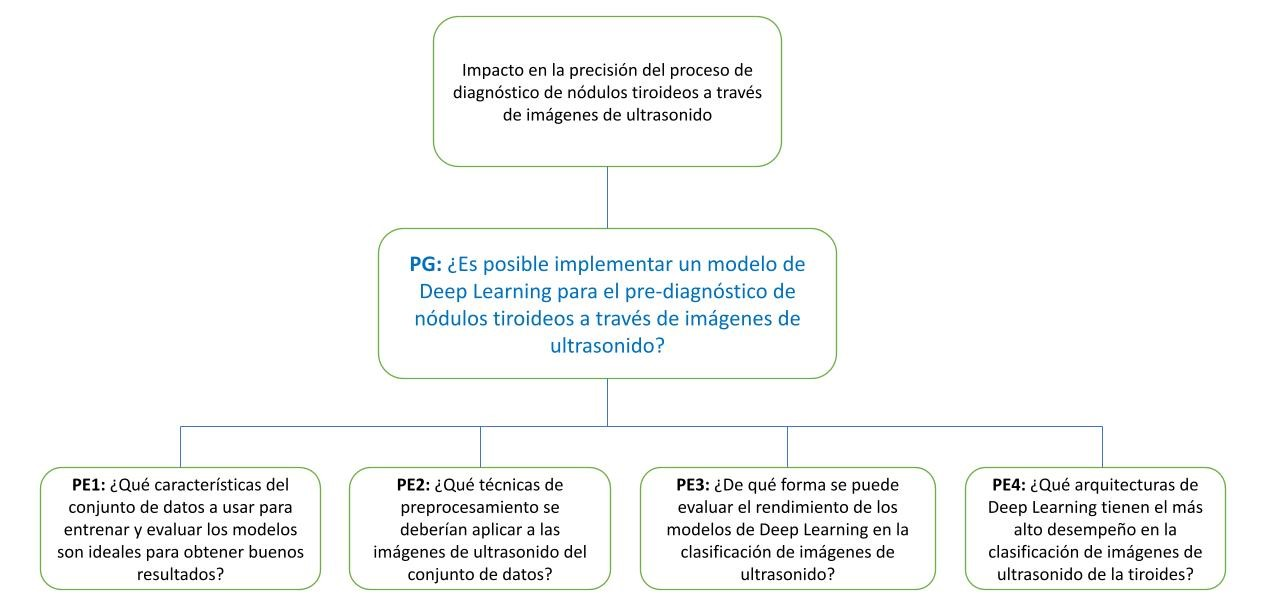
\includegraphics[width=1.05\textwidth]{anexos/arb_problemas.jpg}
			%\caption{Fuente: Elaboración propia}
		\end{center}
	\end{figure}
	\clearpage
	
	\section{Árbol de Objetivos}
	%\chapter*{Árbol de Objetivos}
	%\addcontentsline{toc}{section}{Árbol de Objetivos}
	%\renewcommand{\thechapter}{A}
	\label{anexo2}
	\begin{figure}[h]
		\begin{center}
			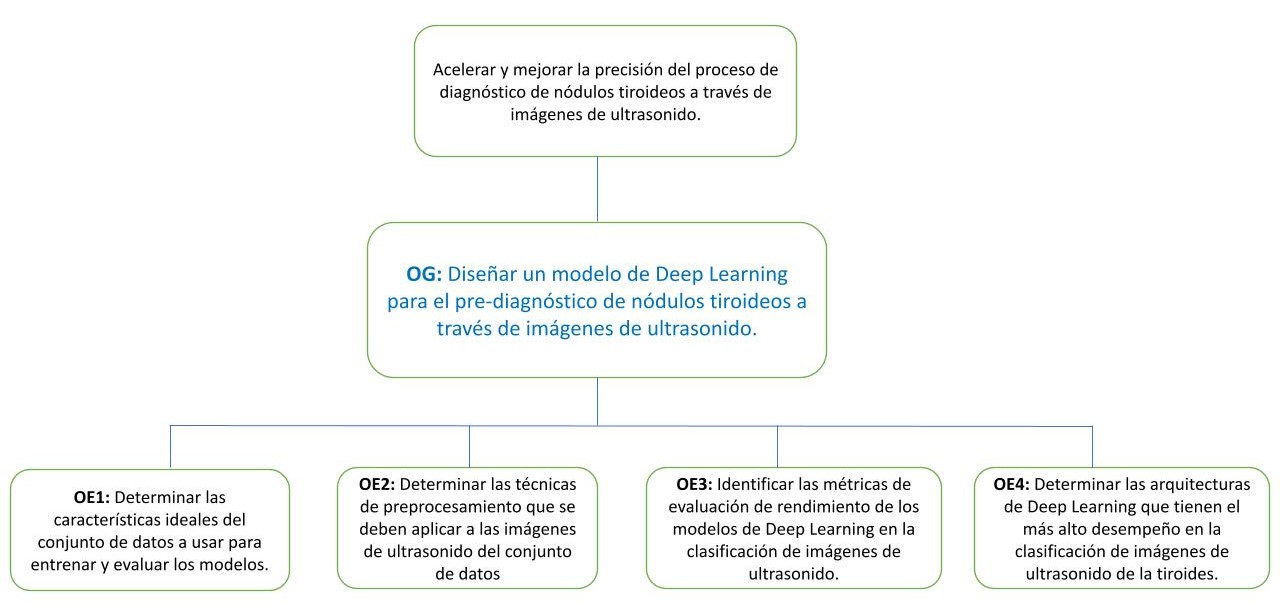
\includegraphics[width=1.05\textwidth]{anexos/arb_objetivos.jpg}
			%\caption{Fuente: Elaboración propia}
		\end{center}
	\end{figure}
	\clearpage
	
	\begin{landscape}
		\section{Matriz de Consistencia}
		\label{anexo3}
		\begin{longtable}{ p{3.5cm}p{3.5cm}p{3.5cm}p{3cm}p{3cm}p{3cm}p{3cm} }
			%\centering
			\small
			\tabularnewline \specialrule{.1em}{.05em}{.05em}
			\centering{Título de la tesis} & \multicolumn{6}{p{15cm}}{Diseño de un modelo de Deep Learning para el pre-diagnóstico de nódulos tiroideos a través de imágenes de ultrasonido}
			\tabularnewline \specialrule{.1em}{.05em}{.05em}
			\Centering{Problema General}& \Centering{Objetivo General} & \Centering{Hipótesis General} & \Centering{Variables} & \Centering{Método} \\
			\specialrule{.1em}{.05em}{.05em}
			{\ProblemaGeneral} & { \ObjetivoGeneral} & {\HipotesisGeneral} & {

				Dependiente: Pre-diagnóstico de nódulos tiroideos. Independiente: Modelo de Deep Learning.

			} \\
			\cline{1-4}
			\Centering {Problemas Específicos} & \Centering {Objetivos Específicos} & \Centering {Hipótesis Específicas} & \Centering {Variables} \\ %& \Centering {Método} \\
			\cline{1-4}
			{\Pbone} & {\Objone} & {\Hone} & {

				Dependiente: Desarrollo del modelo de Deep Learning. Independiente: Las características del conjunto de datos.

			} & \multirow{6}{3cm}{
				
				\centering Tipo de Investigación: Experimental. Alcance de la investigación: Explicativo.
			
			} \\
			\cline{1-4}
			{\Pbtwo} & {\Objtwo} & {\Htwo}  & {
				
				Dependiente: Desempeño del modelo de Deep Learning. Independiente: Técnicas de preprocesamiento.
			
			} \\ % & {aa } \\
			\cline{1-4}
			{\Pbthree} & {\Objthree} & {\Hthree}  & { 
				
				Dependiente: Comparación de modelos en la tarea de clasificación de imágenes de ultrasonido. Independiente: Las métricas de evaluación de rendimiento.
				
			} \\ % & {aa } \\
			\cline{1-4}
			{\Pbfour} & {\Objfour} & {\Hfour}  & { 
				
				Dependiente: Desempeño en la clasificación de imágenes de ultrasonido. Independiente: Las arquitecturas de Deep Learning.
			
			} \\ % & { aa} \\
			\specialrule{.1em}{.05em}{.05em}
		\end{longtable}
	\end{landscape}
	\clearpage
	